\section*{Aufgabe 1a)}
In der ersten Teilaufgabe war zu zeigen, dass die gegebene Relation
$$C \equiv i(\hat{p} \hat{x} - \hat{x}\hat{p}) = 1$$ für beliebige, exakte Matrizen
nicht exakt gilt. Dafür wird die Spur der Operatoren in Matrixdarstellung
untersucht, für die diese Relation auch gelten muss, da es sich bei beiden Ausdrücken
um Diagonale Matrizen handelt. 
\begin{eqnarray}
Tr(\hat{p} \hat{x} - \hat{x}\hat{p}) &=& Tr(1) = N\\
&=& Tr(\hat{p} \hat{x}) - Tr(\hat{x}\hat{p})
\end{eqnarray}
Da für beliebige Matrizen $A,B$ gilt: $$Tr(A\cdot B) = Tr(B\cdot A)$$ ist der
obige Ausdruck null:
\begin{eqnarray}
Tr(\hat{p} \hat{x} - \hat{x}\hat{p}) &=& 0 \neq N
\end{eqnarray}
Da die Spuren des Orts-Impuls-Kommutators und der Einheitsmatrix nicht gleich sind,
ist auch die gegebene Relation selbst nicht exakt erfüllt.

\section*{Aufgabe 1b)}
In der Vorlesung wurde ein Ausdruck für $δ_{ij}$ über eine Fouriertransformation
gegeben: $$δ_{ij} = \frac{1}{N}\sum_p\exp(ip(x_k-x_l)).$$ 

Eine Wellenfunktion, die man sich aus Einträgen dieser Matrix zusammengesetzt
vorstellen kann, lässt sich demnach wie folgt über eine Fouriertransformation
darstellen:
\begin{eqnarray}
Ψ_k &=& \sum_l δ_{kl} = \frac{1}{L}\sum_p\tilde{Ψ}_p e^{ipx_k}\\
\tilde{Ψ}_p &=& a\sum_l Ψ_l e^{ipx_l}\\
\end{eqnarray}
Nun kann untersucht werden, wie ein quantenmechanischer Impulsoperator in
Matrixdarstellung auf eine solche Wellenfunktion wirkt:
\begin{eqnarray}
\hat{p}_{kl}Ψ_l &=& \frac{\hbar}{i}\frac{∂}{∂x_k}Ψ_l = \frac{1}{L}\sum_{p} p e^{ipx_k}\tilde{Ψ}_{p,l}\\
&=& \frac{a}{L}\sum_p p e^{ip(x_k-x_l)}Ψ_l
\end{eqnarray}
Über einen Koeffizientenvergleich kann nun $\hat{p}_{kl}$ unter Ausnutzung von
$N = La$ identifiziert werden:
\begin{eqnarray}
\hat{p}_{kl} = \frac{1}{N}\sum_p p e^{ip(x_k-x_l)}
\end{eqnarray}
Wenn man schließlich noch verwendet, dass es sich bei $\hat{p}$ um einen symmetrischen
Operator handelt, lässt sich diese Formel noch weiter vereinfachen:
\begin{eqnarray}
\hat{p}_{kl} = \frac{2i}{N}\sum_{|p|} |p| e^{i|p|(x_k-x_l)}
\end{eqnarray}
Diese Formel wurde schließlich implementiert. Der Quellcode für die Funktion, 
die den $p$-Operator generiert, ist in \lref{fkt} dargestellt.
\lstinputlisting[label=lst:fkt,caption={ho\_fou.m}]{../code/ho_fou.m}

Diese Funktion wird wie in \lref{1a} aufgerufen:
\lstinputlisting[lastline=2,label=lst:1a,caption={steuerung.m}]{../code/steuerung.m}

\section*{Aufgabe 1c)}
Das resultierende $C$, wie es mit Hilfe der Rückgabewerte des Aufrufs is Aufgabe 1b)
aus den zurückgegebenen Werten von $x$ und $p$ berechnet werden kann, lässt sich,
wie in \lref{1c} gezeigt, plotten, woraus \fref{mesh_c} resultiert.

\lstinputlisting[firstline=5,lastline=16,firstnumber=5,label=lst:1c,caption={steuerung.m}]{../code/steuerung.m}

\begin{figure}[htb]
  \centering
  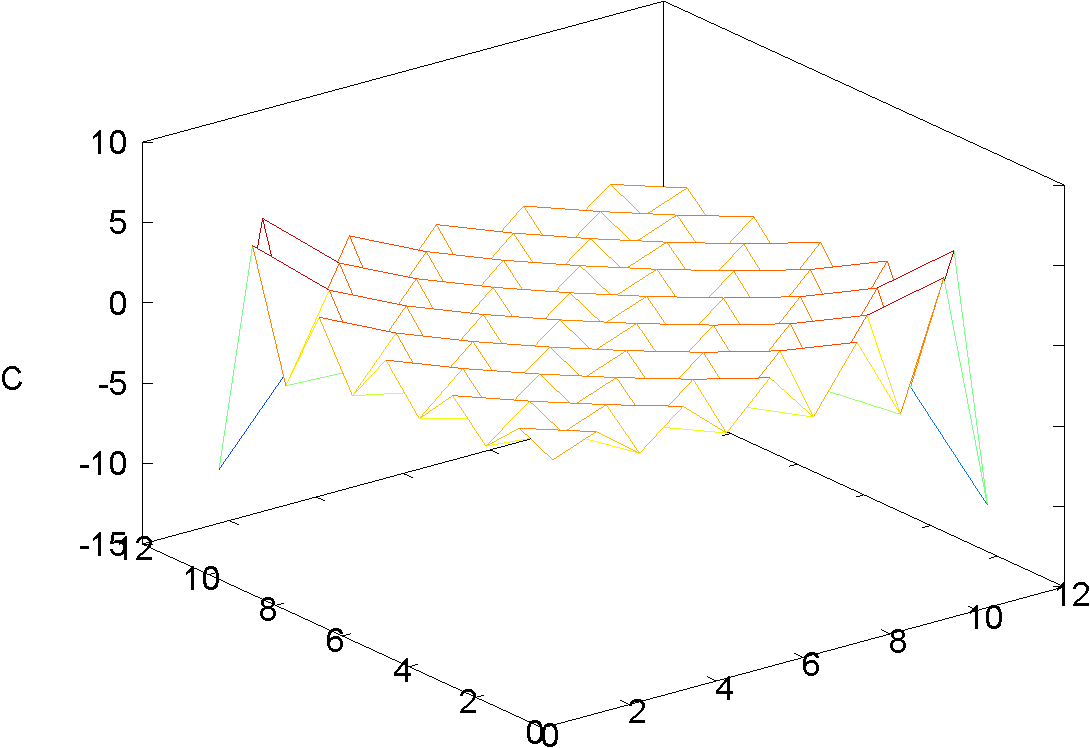
\includegraphics[width=0.8\columnwidth,keepaspectratio]{../tmp/mesh_c-crop}
  \caption{Mesh-Plot von $C$}
  \label{fig:mesh_c}
\end{figure}

Wie man erkennen kann, schwanken die Einträge in $C$ in der Größenordnung von 1, sodass
die Relation als näherungsweise erfüllt gelten kann.

\section*{Aufgabe 1d)}
Um zu überprüfen, ob die gegebene Relation $<a|C-1|b>=0$ erfüllt ist, wurden normierte Gaußfunktionen
erstellt und mit diesen wurden die gesuchten Skalarprodukte berechnet. Der entsprechende Code
ist in \lref{1d} dargestellt.

\lstinputlisting[firstline=19,lastline=36,firstnumber=19,label=lst:1d,caption={steuerung.m}]{../code/steuerung.m}

Der Wert von σ wurde frei gewählt.

Um zu überprüfen, inwieweit diese Ergebnisse null ergeben, wurde erneut ein Mesh-Plot der resultierenden
Matrix erstellt, was in \fref{diff} zu sehen ist.

\begin{figure}[htb]
  \centering
  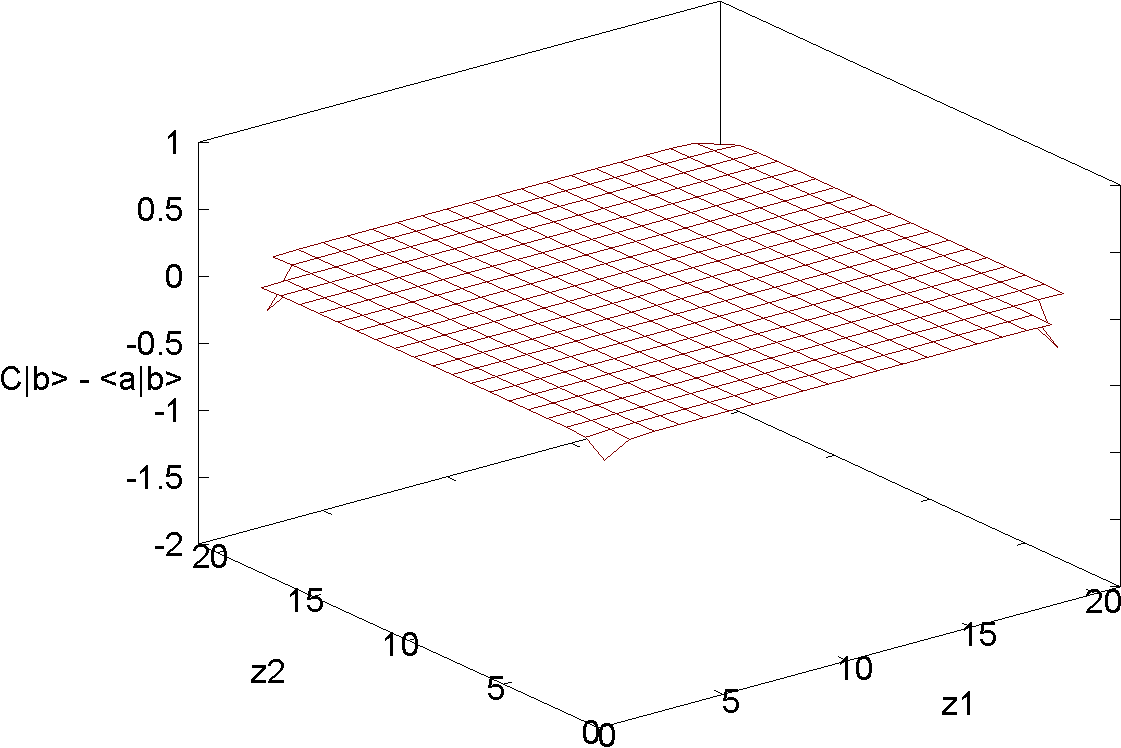
\includegraphics[width=0.8\columnwidth,keepaspectratio]{../tmp/Diff-crop}
  \caption{Mesh-Plot von $C-1$}
  \label{fig:diff}
\end{figure}

Wie man erkennen kann, sind fast alle Einträge annähernd null, abgesehen von den vier Randpunkten.
Doch auch diese sind immernoch in der Größenordnung von $0.1$ verschieden von null, sodass die zu 
untersuchende Relation als erfüllt gelten kann.

\section*{Aufgabe 1e)}
Schließlich war ein Plot für den gegebenen Ausdruck mit variablem σ zu erstellen. Dieser ist in 
\fref{plot1e} dargestellt.

\begin{figure}[htb]
  \centering
  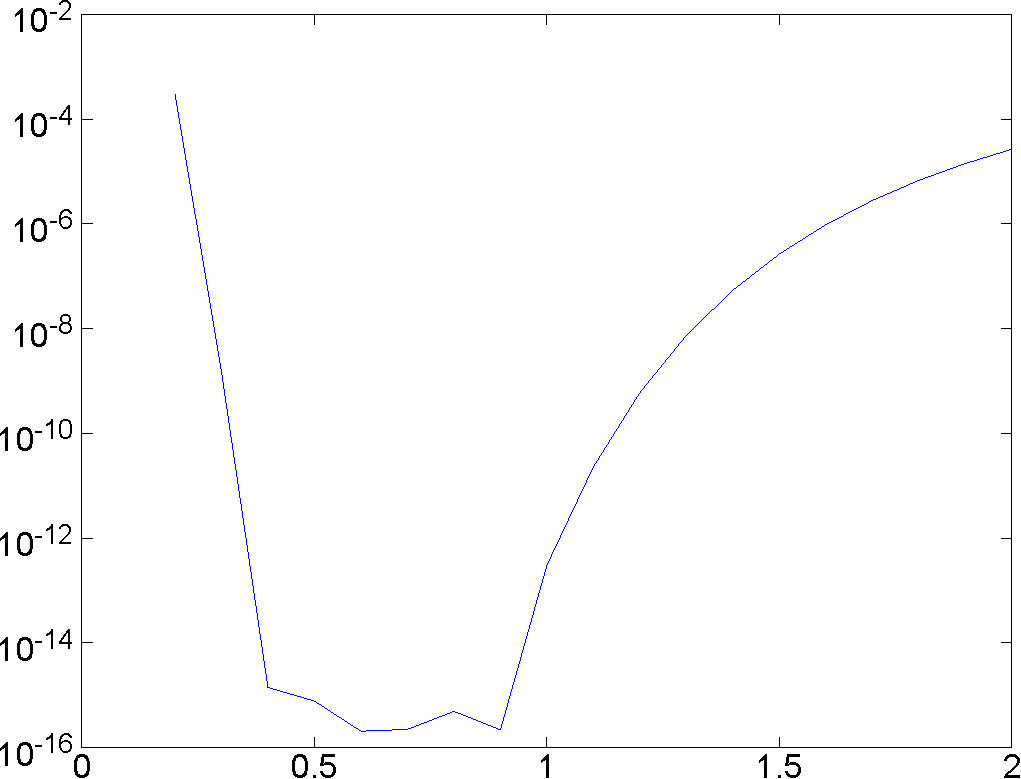
\includegraphics[width=0.8\columnwidth,keepaspectratio]{../tmp/plot-crop}
  \caption{Erwartungswert von $C-1$ mit $z=5$ in Abhängigkeit von σ}
  \label{fig:plot1e}
\end{figure}

Der Code, der für die Erstellung verwendet wurde, ist in \lref{1e} dargestellt.
\lstinputlisting[firstline=48,lastline=59,firstnumber=59,label=lst:1e,caption={steuerung.m}]{../code/steuerung.m}

Wie man in \fref{plot1e} erkennen kann, ist für $σ=0.2$ der Erwartungswert von $C-1$ mit ungefähr $10^{-4}$
relativ groß, während er für $σ=0.3$ schon annähernd in der Größenordnung der Mascheninengenauigkeit liegt.
Eine Erklärung für den Wert bei $σ=0.2$ könnte sein, dass hier die sehr schmale Gaußfunktion durch eine ungünstige 
Einteilung der $N_x$ Gitterpunkte schlecht ausgewertet wird. Wenn man beispielsweise den Wert für $N_x$ auf 201 
setzt, so sinkt für diesen σ-Wert der Erwartungswert auf ca. $10^{-15}$ und liegt somit im selben Bereich wie für die 
folgenden σ-Werte. Für $σ>0.9$ steigt der Erwartungswert schnell an, was wiederum eine Folge der Diskretisierung 
durch das Gitter darstellt, wobei für große $N$ der Wert von $C$ gemäß Gl. (3) stark verschieden vom Einheitsoperator
ist und somit für die große Abweichung verantwortlich ist.